\documentclass[10pt]{article}
\usepackage{graphicx}
\usepackage{siunitx}
\usepackage{listings}
\usepackage{color}
\usepackage{mathptmx}
\usepackage[export]{adjustbox}
\usepackage{float}
\usepackage{amsmath}
\usepackage[a4paper,bindingoffset=0.1in,%
            left=1in,right=1in,top=1in,bottom=1in,%
            footskip=.25in]{geometry}
\title{EE314 Digital Electronics Laboratory Term Project Proposal Report \\* FPGA Based Oscilloscope}
\date{2018\\ May}
\author{Ekin Yılmaz - 2094738 Nail Tosun - 2094563\\ Electrical and Electronics Engineering Department, METU}
\begin{document}
\maketitle
\section*{Introduction}
For this purpose, a system which consists of a ADC measuring module to quantize the signal, a data storage module where the transmitted quantized data is stored, a computation module that performs the required measurements and calculations to determine frequency, peak-to-peak voltage, waveform, rms voltage, and offset voltage and finally a VGA display module where the visualization of the results is realized, is designed. Related block diagram of the overall system can be seen in Figure 1. In addition to these modules, there will be also a mode selection input which decides whether the oscilloscope will measure in AC mode od DC mode. According to the decision made, entire signal will be visualized for DC mode or DC value will be subtracted first then the signal will be demonstrated in AC mode. This mode selection part will be realized via switches on the FPGA board. Finally, there must be also adjustable time/div, volt/div and auto scale option too. Those arrangements will be done by using push buttons on the board.

\begin{table}[H]
\centering
\caption{The required measurements that the designed oscilloscope can achieve}
\label{my-label}
\begin{tabular}{ccc}
Parameter & \begin{tabular}[c]{@{}c@{}}Max-Min\\   Values\end{tabular} & Resolution \\
Frequency & DC – 20kHz                                                 & 10 Hz      \\
Vpp       & 0 to 5 Volts                                               & 20 mV      \\
Vrms      & 0 to 5 Volts                                               & 20 mV      \\
Voffset   & 0 to 5 Volts                                               & 20 mV     
\end{tabular}
\end{table}
\section*{Working Principle of Design}
\subsection*{ADC Analog to Digital Converter}
The input signal coming from the signal generator is an analog signal and has to be converted to digital by the ADC. Embedded ADC on the board will be used in this part. Sampling rate of the ADC is crucial since it determines the functioning of all the remaining modules.
\subsection*{Storage Unit (DRAM)}
To store the serial input data first it must be converted to parallel. Details about FIFO structure will be mentioned in final report with more detail.
\subsection*{Computation Module}
\subsubsection*{Frequency Measurement}
Determining a suitable trigger value the difference between first and third point must be denoted as one period no matter what type of waveform is given.
\subsubsection*{Peak to Peak Voltage Detection}
In each cycle obtained serial data must be compared to the previous data and when the maximum value is reached, peak voltage must be determined.
\subsubsection*{RMS Voltage Detection}
Starting the design, an RMS voltage measurement module is designed first since it will also be a crucial part of AC DC selection module too. For this purpose, an algorithm that firstly takes the square then sums up the given serial input for a given sampling period and then takes the average of the total value by dividing the sum to total number of cycles is designed first. The output of this module which takes the average of the given serial input is connected to another module that simply takes the square root of the average value and as a final result RMS value is obtained. The methods that are used previously in laboratory sessions in the subject of interconnection of the modules are used in this step.
\subsubsection*{Offset Voltage Measurement}
RMS module can also be helpful here. We can simply find the offset value by dividing the sum of the sampled inputs to number of the samples taken. A basic average finder will work and produce a very important data to be used further in the mode selection when subtracting DC value from the total input.
\subsection*{VGA module}
Plotting will be done in this module. First an image buffer must be created to store each data line coming from the computation module. Also, since the screen must be renewed once in one second clock of the VGA module must be arranged accordingly using a frequency divider.
\begin{figure}[H]
  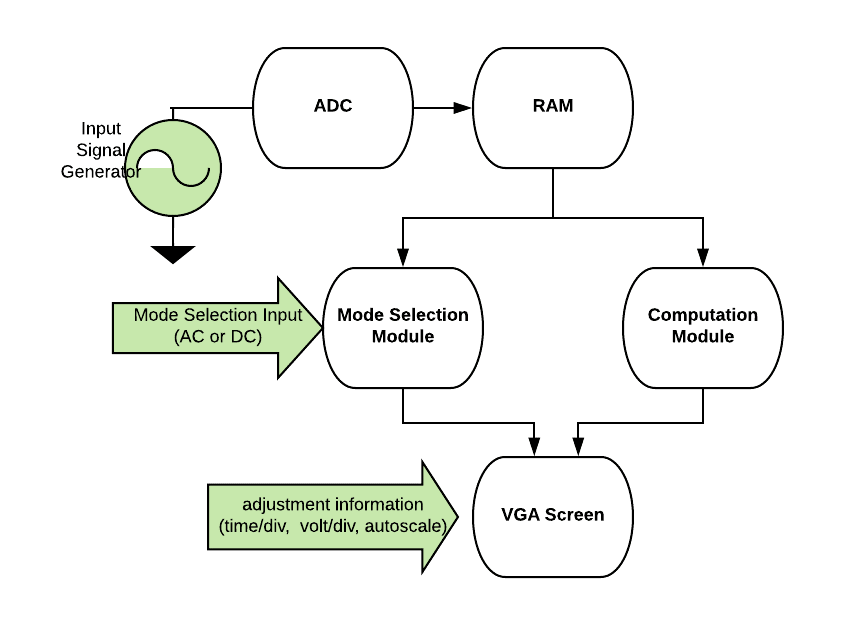
\includegraphics[scale=0.4, center]{blockdiagram}
  \caption{Block diagram of the overall system}
  \label{fig:zero}
\end{figure}
\section*{Equipment}
VGA connector, VGA display screen, De1-SoC FPGA development board.
Mainly the VGA outputs and embedded ADC of the board will be used in this project. Input signals will be applied from the ADC header and the output will be taken from the VGA output of the development board for visualization.
\section*{Rms voltage measurement unit}
Starting the design, an RMS voltage measurement module is designed first since it will also be a crucial part of AC DC selection module too.

Discrete RMS formula is following;
\[V_{rms}=\sqrt{\frac{1}{N}\sum\limits_{i=0}^{N-1}V_i^2}\]
Then we firstly took square every serial in values. This module HDL code is following;
\begin{lstlisting}[language=Verilog, caption=Square module]
module square(clk,serial_in,square_out);
input clk;
input [11:0] serial_in; 
output reg [31:0] square_out;
always @(posedge clk)
begin
square_out<=serial_in*serial_in;
end
endmodule

\end{lstlisting}

Then we sum squares of serial in values after to one period and divide the period $N$ for mean value of squares. (Frequency of the signal is an    \textit{input} for this module). HDL code is following;
\begin{lstlisting}[language=Verilog, caption=Averaging module]
module rms_finder(clk, freq, average, serial_in);
input clk;
input [11:0] serial_in;
input [31:0] freq;
output reg [31:0] average;
integer index,N,dum_index,sum; 
initial
begin
sum <= 0;
N <= 0;
index <= 0;
average <= 0;
dum_index <= 1;
end
always @(posedge clk)
begin
	N = 8; //for testing normally fsampling/f
	if (index<N)
		begin
		sum <= sum + serial_in;
		index <= index+1;
		end
	else if(index==N)
	begin
	dum_index <= dum_index + 1;
	average <= sum/(N*dum_index);
	index <= index +1;
	dum_index <= dum_index + 1;
	end
	else index <= 0;
end
endmodule

\end{lstlisting}

Then we write another module that simple take square root of the input. HDL code of this module is following;

\begin{lstlisting}[language=Verilog, caption=Square-root module]
module m(clk, mean_input, rms);
input clk;
input [11:0] mean_input;
output reg [11:0] rms;
reg [11:0]temp=1;

always@(posedge clk)
begin
	if((temp*temp)>=mean_input)
		rms<=temp;
   else
      temp<=temp+1;
  end
endmodule
\end{lstlisting}

\begin{lstlisting}[language=Verilog,caption=Top level design]
module top(clk,serial_in,freq,rmsfindresult);
input clk;
input [11:0]serial_in;
input [31:0] freq;
output  reg [11:0] rmsfindresult;
wire[11:0] square_out,average,rms,serial_in_sq;
reg [11:0] serial_in_sq,mean_input;
square(.clk(clk),
.serial_in(serial_in),
.square_out(square_out));
Mean(.clk(clk),
.serial_in_sq(square_out),
.freq(freq),
.average(average));
root(.clk(clk),
.mean_input(average),
.rms(rms));
always begin
serial_in_sq <= square_out;
mean_input <= average;
rmsfindresult <= rms;
end
endmodule
\end{lstlisting}

\section*{Simulation Results}
\begin{figure}[H]
  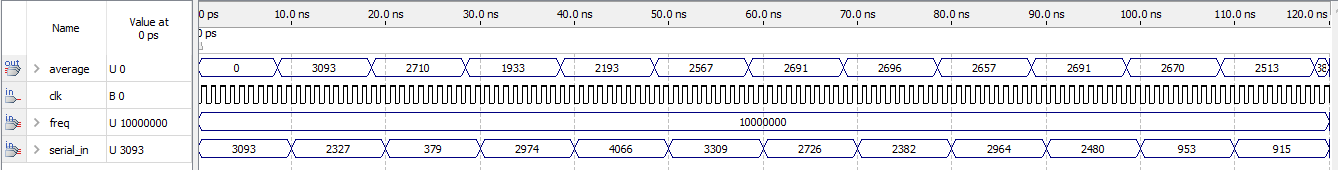
\includegraphics[scale=0.5, center]{Mean_finder}
  \caption{Simulation results of mean-finder}
  \label{fig:zero}
\end{figure}


\begin{figure}[H]
  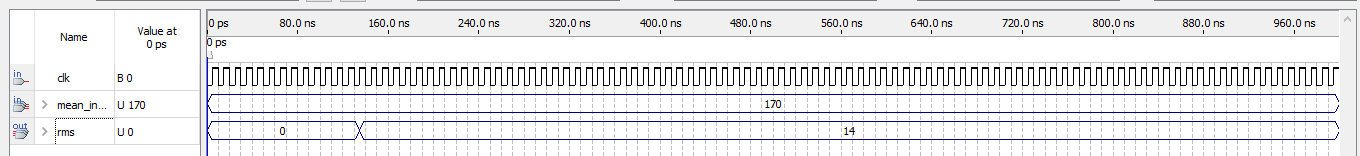
\includegraphics[scale=0.5, center]{Rms_out}
  \caption{Simulation results of square root module}
  \label{fig:zero}
\end{figure}

\begin{figure}[H]
  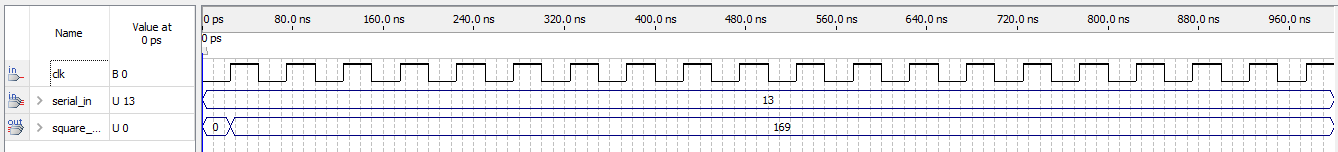
\includegraphics[scale=0.5, center]{square}
  \caption{Simulation results of square module}
  \label{fig:zero}
\end{figure}
\end{document}
